\documentclass[a4paper,11pt]{article}

% ---------- Кодировка и язык ----------
\usepackage[utf8]{inputenc}
\usepackage[T2A]{fontenc}
\usepackage[english,russian]{babel}

% ---------- Геометрия страницы ----------
\usepackage[margin=2.5cm]{geometry}

% ---------- Математика ----------
\usepackage{amsmath,amssymb,amsthm,mathtools}

% ---------- Оформление ----------
\usepackage{enumitem}
\usepackage{booktabs}
\usepackage{graphicx}
\graphicspath{{figures/}}
\usepackage{float}
\usepackage{xcolor}
\usepackage[colorlinks=true,linkcolor=blue,urlcolor=blue,citecolor=blue]{hyperref}
\usepackage{cleveref}
\newcommand{\lean}[1]{\mbox{\path{#1}}}

% ---------- Теоремы и окружения ----------
\theoremstyle{plain}
\newtheorem{theorem}{Теорема}[section]
\newtheorem{lemma}[theorem]{Лемма}
\newtheorem{proposition}[theorem]{Утверждение}
\newtheorem{corollary}[theorem]{Следствие}

\theoremstyle{definition}
\newtheorem{definition}[theorem]{Определение}

\theoremstyle{remark}
\newtheorem*{remark}{Замечание}

% ---------- Полезные макросы ----------
\newcommand{\R}{\mathbb{R}}
\newcommand{\abs}[1]{\left\lvert #1 \right\rvert}
\newcommand{\norm}[1]{\left\lVert #1 \right\rVert}
\newcommand{\set}[1]{\left\{ #1 \right\}}
\newcommand{\ip}[2]{\langle #1, #2\rangle}
\newcommand{\Rpp}[1][2]{\R^{#1}_{++}}
\newcommand{\Rp}[1][2]{\R^{#1}_{+}}
\DeclareMathOperator{\conv}{conv}
\DeclareMathOperator{\cone}{cone}
\DeclareMathOperator{\Sp}{Sp}
\DeclareMathOperator{\dev}{dev}
\newcommand{\OPT}{\mathrm{OPT}}
\newcommand{\BOX}{\mathrm{BOX}}
\newcommand{\LB}{\mathrm{LB}}
\newcommand{\UB}{\mathrm{UB}}
\newcommand{\todo}[1]{\textcolor{red}{\textbf{TODO:} #1}}

\title{Наименьшее возмущение цен в метрике $\ell_p$:\\ точный алгоритм с оракулом коробки и сертификатами отказа}
\date{}

\begin{document}
\maketitle

\section{Постановка}

Всюду $d\ge2$. Обозначения те же, что в основных заметках (\texttt{latex/notes.tex}) и в \texttt{price-perturbation/tex/price-perturbation.tex}. Цены $P=\set{p_t\in\Rpp[d]}_{t\in[T]}$, выпуски $y\in\Rp[T]$. Используется критерий слабой разрешимости: $y$ слабо разрешим при ценах $Q$ тогда и только тогда, когда $y\in\cone\set{\mathbf 1_S\mid S\in\widehat{\Sp}(Q)}$. Операции над векторами покоординатные.

\paragraph{Стоимость.} Отклонение новой цены $q$ от $p$ измеряется одной из двух метрик:
\[
    \dev(q,p)=\ln q-\ln p\quad(\text{логарифмическая}),\qquad \dev(q,p)=q/p-1\quad(\text{относительная}).
\]
Пусть $c^i_t>0$~--- веса и $1\le p\le\infty$. Стоимость набора $Q$ есть одна взвешенная норма $\ell_p$ всего вектора отклонений всех цен всех лет:
\[
    C_p(Q):=\norm{c\circ\dev(Q,P)}_p,\qquad \OPT_p:=\inf\set{C_p(Q)\mid y\text{ слабо разрешим при }Q}.
\]
Относительная метрика~--- стандартная мера ошибки цен в литературе о выявленных предпочтениях \cite{Varian1985,DemuynckRehbeck2023}. При малых отклонениях метрики совпадают с точностью до второго порядка.

\paragraph{Коробки.} Положим $g(z)=e^z$ для логарифмической метрики и $g(z)=1+z$ для относительной. Полуширинам $\alpha,\beta\in\Rp[d\times T]$ (для относительной метрики $\alpha<1$) сопоставим коробку с углами $a_t:=p_t\circ g(-\alpha_t)$, $b_t:=p_t\circ g(\beta_t)$ и набор углов $W(\alpha,\beta):=(a_1,\dots,a_T,b_1,\dots,b_T)$. Запрос $\BOX(\alpha,\beta)$: существует $w\in\cone\set{\mathbf 1_S\mid S\in\widehat{\Sp}(W(\alpha,\beta))}$ с $w(a_t)\ge y_t\ge w(b_t)$ при всех $t$. По теореме об углах (\texttt{price-perturbation.tex}, \lean{box_iff}) $\BOX(\alpha,\beta)$ равносилен существованию $Q$ с $a_t\le q_t\le b_t$, при котором $y$ слабо разрешим. Точный оракул коробки~--- генерация столбцов с точной геометрией (\texttt{price-perturbation/perturb/exact\_oracle.py}). Он полиномиален по числу вызовов оракула слабой разрешимости. При $d\ge3$ сама проверка слабой разрешимости NP-трудна.

\paragraph{Результаты.}
\begin{enumerate}[label=(\roman*)]
    \item Задача равносильна минимизации возрастающей функции $\norm{c\circ(\alpha+\beta)}_p$ на замкнутом вверх множестве полуширин, проходящих один запрос $\BOX$ (теорема~\ref{thm:reduction}). Оптимум однонаправлен по годам (теорема~\ref{thm:onesided}).
    \item Отказ оракула сопровождается сертификатом: вектором Фаркаша и конечным набором покрытий. Отказ сохраняется во всякой коробке, где эти покрытия присутствуют (теорема~\ref{thm:certificate}). Отсюда отсечения <<хотя бы одно покрытие исчезло>>. В относительной метрике они линейны при фиксированной выпуклой комбинации.
    \item Алгоритм~--- внешняя аппроксимация полиблоками для монотонной оптимизации \cite{Tuy2000,TuyAlKhayyalThach2005} с мастер-задачей MILP вместо перебора вершин и с комбинаторными отсечениями Бендерса из сертификатов \cite{CodatoFischetti2006}. Нижняя граница всегда верна, верхняя всегда достигается проверенным рациональным решением. При любом $\varepsilon>0$ алгоритм останавливается с относительным зазором не больше $\varepsilon$ (теорема~\ref{thm:algo}).
\end{enumerate}
Сведение к коробкам (обе метрики), однонаправленность, доминирование, теорема о сертификате отказа и оценка упаковки проверены в Lean (\texttt{lean/L1Perturbation/Reduction.lean}, без \texttt{sorry}, стандартные аксиомы).

\paragraph{Литература.} Меры согласия для тестов выявленных предпочтений возмущают по одному скаляру на наблюдение (индексы Африата и Варьяна). Индекс Африата вычисляется бисекцией по критическим значениям, индекс Варьяна NP-труден, индекс Хаутмана--Макса неаппроксимируем \cite{Cherchye2014}. Наш максимум по годам~--- аналог индекса Африата, он решён в \texttt{price-perturbation}. Возмущение каждой цены с нормой $\ell_1$ рассмотрено для GARP в \cite{DemuynckRehbeck2023}: там это один MILP, так как условие GARP линейно по ценам при данных количествах. В нашей задаче свидетели латентны, а проверка разрешимости при $d\ge3$ NP-трудна. Поэтому один MILP невозможен, и задача разбивается на мастер-задачу и точный оракул, как перебор циклов с покрытием множествами в \cite{DeanMartin2016}.

\section{Сведение к коробкам}

\begin{theorem}[сведение к коробкам]\label{thm:reduction}
    Для обеих метрик и $1\le p\le\infty$
    \[
        \OPT_p=\inf\Bigl\{\norm{c\circ(\alpha+\beta)}_p\;\Big|\;\alpha,\beta\ge0,\ \BOX(\alpha,\beta)\Bigr\}.
    \]
    Если $\BOX(\alpha,\beta)$, то в коробке есть $Q$ со слабой разрешимостью $y$ и $\abs{\dev(q_t,p_t)}\le\max(\alpha_t,\beta_t)$ при всех $t$. Множество $\set{(\alpha,\beta)\mid\BOX(\alpha,\beta)}$ замкнуто вверх.
\end{theorem}

\lean{exists_weakSolvable_iff_boxFeasible_lp}, \lean{exists_weakSolvable_iff_boxFeasible_linf}, \lean{BoxFeasible.mono} (логарифмическая метрика); \lean{exists_weakSolvable_iff_boxFeasible_rel}, \lean{exists_weakSolvable_iff_boxFeasible_rel_lp} (относительная метрика).

\begin{proof}
    Пусть $Q$ допустим и $u_t:=\dev(q_t,p_t)$. Положим $\alpha_t:=u_t^-$, $\beta_t:=u_t^+$. Функция $\dev(\cdot,p)$ возрастает, поэтому $a_t=\min(p_t,q_t)\le q_t\le\max(p_t,q_t)=b_t$, и $\BOX(\alpha,\beta)$ выполнен по теореме об углах. При этом $\alpha_t+\beta_t=\abs{u_t}$.

    Обратно, по теореме об углах в коробке есть допустимый $Q$. Для точки $q$ коробки $\dev(q,p)\in[-\alpha,\beta]$ покоординатно: $\dev(\cdot,p)$ возрастает и $\dev(p\circ g(\pm z),p)=\pm z$. Значит, $\abs{\dev(q,p)}\le\max(\alpha,\beta)\le\alpha+\beta$. Монотонность: точка меньшей коробки лежит в большей.
\end{proof}

\paragraph{Стоимость коробки.} Величина $\overline C(\alpha,\beta):=\norm{c\circ\max(\alpha,\beta)}_p$ ограничивает сверху стоимость решения, построенного по коробке. Её достаточно для верхней границы алгоритма: решение строится один раз, в конце.

\section{Однонаправленность}

\begin{theorem}[однонаправленность]\label{thm:onesided}
    \begin{enumerate}[label=(\alph*)]
        \item Для всякого допустимого $Q$ найдётся допустимый $Q'$, у которого для каждого $t$ либо $q'_t\le p_t$, либо $q'_t\ge p_t$, и $\abs{\dev(q'_t,p_t)}\le\abs{\dev(q_t,p_t)}$ покоординатно.
        \item При $1\le p<\infty$ всякий оптимальный $Q$ однонаправлен.
    \end{enumerate}
\end{theorem}

\lean{exists_oneSigned}, \lean{exists_oneSigned_le}, \lean{exists_lt_of_mixed_lp}.

\begin{proof}
    (a) Коробка $(u^-,u^+)$ содержит $Q$. Путь из $a_t$ через $p_t$ в $b_t$ непрерывен. Построение теоремы об углах даёт на нём точку $q'_t$ до $p_t$ или после. В первом случае $q'_t\le p_t$ и $\abs{\dev}\le u^-_t$, во втором $q'_t\ge p_t$ и $\abs{\dev}\le u^+_t$.

    (b) Стоимость $C_p^p$ аддитивна по координатам. Если у года есть сдвиги разных знаков, то по (a) один из двух положительных вкладов исчезает, и стоимость строго падает.
\end{proof}

Поэтому в мастер-задаче вводится знак года $\sigma_t\in\set{0,1}$ с $\alpha_t\le z^{\max}\sigma_t$, $\beta_t\le z^{\max}(1-\sigma_t)$.

\section{Покрытия и сертификат отказа}

\begin{definition}
    Пусть $W$~--- набор точек. Пара $(t,A)$, $t\notin A$, называется \textit{покрытием в $W$}, если некоторая выпуклая комбинация $\sum_{s\in A}\mu_sW_s$ строго меньше $W_t$ по всем координатам.
\end{definition}

\begin{proposition}[покрытие]\label{prop:cover}
    Если $(t,A)$~--- покрытие в $W$ и $S\in\widehat{\Sp}(W)$ содержит $t$, то $S\cap A\ne\varnothing$. В частности, если $y$ слабо разрешим при $Q$ и $(t,A)$~--- покрытие в $Q$, то $y_t\le\sum_{s\in A}y_s$.
\end{proposition}

\lean{meets_of_conv_lt}, \lean{le_sum_of_conv_lt}, \lean{le_of_lt}.

\begin{proof}
    Пусть $S\cap A=\varnothing$. Свидетель $\xi\ge0$, $\xi\ne0$ индекса $t$ даёт $\ip{\xi}{W_s-W_t}\ge0$ при $s\in A$. Взвесим коэффициентами $\mu_s$: $\ip{\xi}{\sum_s\mu_sW_s-W_t}\ge0$. Но вектор в скобке строго отрицателен, и произведение отрицательно. Второе утверждение: функция $x\mapsto\sum_{s\in A}x_s-x_t$ неотрицательна на образующих конуса.
\end{proof}

Точный оракул решает задачу о конусе генерацией столбцов. Подзадача ищет множество $S$ с наименьшим $\lambda(S)$ среди множеств, удовлетворяющих неравенствам покрытий $x_t\le\sum_{s\in A}x_s$. Покрытия добавляются лениво и проверяются точно, в рациональной арифметике. При ответе <<нет>> оракул возвращает вектор Фаркаша $\lambda\in\mathbb Q^{2T}$ и набор $\mathcal C$ покрытий в $W$, такие что
\begin{enumerate}[label=(F\arabic*)]
    \item $\sum_{\lambda_r<0}\abs{\lambda_r}\,\mathrm{lo}_r-\sum_{\lambda_r>0}\lambda_r\,\mathrm{hi}_r>0$, где $\mathrm{lo},\mathrm{hi}$~--- границы запроса ($\mathrm{lo}(a_t)=y_t$, $\mathrm{hi}(b_t)=y_t$, остальные $0$ и $\infty$);
    \item $\lambda(S)\ge0$ для всякого $S\subset[2T]$, удовлетворяющего всем неравенствам покрытий из $\mathcal C$.
\end{enumerate}
Условие (F2) проверяется одной задачей $0/1$ с целыми весами. Границы зависят только от $y$, а не от коробки.

\begin{theorem}[сертификат отказа]\label{thm:certificate}
    Пусть $(\lambda,\mathcal C)$ удовлетворяет (F1), (F2). Если все пары из $\mathcal C$ являются покрытиями в $W(\alpha',\beta')$, то $\BOX(\alpha',\beta')$ не выполнен.
\end{theorem}

\lean{not_boxCone_of_certificate}.

\begin{proof}
    По утверждению~\ref{prop:cover} всякое $S\in\widehat{\Sp}(W(\alpha',\beta'))$ удовлетворяет неравенствам покрытий из $\mathcal C$, поэтому $\lambda(S)\ge0$ по (F2). Значит, $\lambda(w)\ge0$ для всех $w$ конуса. Для $w$ с $w\ge\mathrm{lo}$ на строках с $\lambda_r<0$ и $w\le\mathrm{hi}$ на строках с $\lambda_r>0$ имеем $\lambda(w)\le-\bigl(\sum_{\lambda_r<0}\abs{\lambda_r}\mathrm{lo}_r-\sum_{\lambda_r>0}\lambda_r\mathrm{hi}_r\bigr)<0$ по (F1). Противоречие.
\end{proof}

\paragraph{Минимальный конфликт.} Из $\mathcal C$ удаляются пары, пока (F2) сохраняется (удаление блоками, как поиск минимальной несовместной подсистемы в \cite{CodatoFischetti2006}). Остаётся минимальный по включению набор $\mathcal C'$. По теореме~\ref{thm:certificate} всякая допустимая коробка уничтожает хотя бы одно покрытие из $\mathcal C'$.

\paragraph{Отсутствие покрытия.} Если $(t,A)$ не покрытие в $W'$, то для любой $\mu$ из симплекса на $A$ найдётся координата $i$ с
\begin{equation}\label{eq:absent}
    \sum_{s\in A}\mu_s\,W'^i_s\ \ge\ W'^i_t.
\end{equation}
Углы $W'$ имеют вид $p^i\,g(\pm z_j)$, где $z_j$~--- одна из полуширин. В относительной метрике $g$ линейна, и \eqref{eq:absent} при фиксированной $\mu$~--- линейное неравенство по $z$. В логарифмической метрике $e^{z}$ в левой части заменяется кусочно-линейной интерполяцией на $[0,z^{\max}_j]$ (оценка сверху выпуклой функции, двоичные переменные упорядочивают отрезки), а в правой~--- касательными (оценка снизу). Получается ослабление \eqref{eq:absent}, верное для всех допустимых $z$.

\paragraph{Отсечение по покрытиям.} Для минимального конфликта $\mathcal C'$ и выпуклых комбинаций $\mu$ из сертификата (комбинация, на которой покрытие строго меньше $W_t$) в мастер-задачу добавляется дизъюнкция
\[
    \bigvee_{(t,A)\in\mathcal C'}\ \bigvee_{i\in[d]}\ \Bigl[\sum_{s\in A}\mu_sW^i_s(z)\ge W^i_t(z)\Bigr].
\]
Покрытия с $\abs A=1$~--- это доминирование. Для них условие точно линейно в обеих метриках (в логарифмической~--- по логарифмам).

\section{Алгоритм}

\paragraph{Мастер-задача $M_k$.} Переменные $z=(\alpha,\beta)\in[0,z^{\max}]$, $z^{\max}=\UB/c$ (для $\alpha$ в относительной метрике ещё $\alpha<1$), знаки лет $\sigma_t$. Ограничения: однонаправленность; доминирование, необходимое по утверждению~\ref{prop:cover} (лениво, по нарушенным парам); отсечения полиблока; отсечения по покрытиям. Цель $\norm{c\circ(\alpha+\beta)}_p$: при $p=1$ линейная, при $p=\infty$ через $s\ge c^i_tz^i_t$, при $1<p<\infty$ через касательные к $(c^i_tx^i_t/\UB)^p$ (оценка снизу). $\LB$~--- двойственная граница MILP. Это внешняя аппроксимация замкнутого вверх множества кополиблоком: минимум возрастающей функции на нём достигается в собственной вершине, и MILP заменяет перебор вершин алгоритма QA из \cite{TuyAlKhayyalThach2005}.

\paragraph{Шаг $k$.} Пусть $v$~--- точка мастер-задачи, $\norm{\mathbf1}:=\norm{c\circ\mathbf 1}_p$.
\begin{enumerate}
    \item \textit{Запрос с допуском.} $\delta:=\varepsilon\,\UB/(4\norm{\mathbf1})$, запрос в коробке $v+\delta\mathbf 1$. Да: $\UB:=\min(\UB,\overline C)$, где $\overline C\le f(v)+\delta\norm{\mathbf1}$. Допуск нужен потому, что оптимум лежит на вырождениях (совпадениях координат). Точка мастера получена в плавающей арифметике и попадает на совпадение лишь приближённо. Коробка $v+\delta\mathbf1$ накрывает его строго.
    \item \textit{Проекция} \cite[с.~479]{Tuy2000}. $\tau:=(\UB-\LB)/(2\norm{\mathbf1})$. Бисекция по $\lambda\ge\tau$ для коробок $v+\lambda\mathbf1$ (не больше заданного числа запросов). Да в $\lambda_{\rm hi}$: $\UB:=\min(\UB,\overline C)$. Нет в $\lambda_{\rm lo}\ge\tau$: отсечение полиблока по минимальному множеству лет с отказом (удаление лет, лемма об удалении \lean{BoxFeasible.restrict}) и отсечения по покрытиям из сертификатов отказа в коробках шагов 1 и 2.
\end{enumerate}
В конце из лучшей коробки строится рациональное $Q$ (построение теоремы об углах на путях, линейных по ценам). Слабая разрешимость $y$ при $Q$ проверяется независимо, в рациональной арифметике. Ответ: $Q$, $\UB=C_p(Q)$, $\LB$.

\paragraph{Отсечение полиблока.} Пусть $Y$~--- множество лет и $\hat z$~--- полуширины, при которых запрос на годах $Y$ отвечает <<нет>>. Тогда всякая допустимая коробка имеет координату $j$ года из $Y$ с $z_j>\hat z_j$. Иначе по монотонности допустима коробка $\hat z$ на годах $Y$, что противоречит лемме об удалении лет. Отсечение $\bigvee_jz_j\ge\hat z_j$ отрезает вершину кополиблока, как в \cite{Tuy2000,TuyAlKhayyalThach2005}.

\begin{lemma}[упаковка]\label{lem:packing}
    Если точки $z^1,\dots,z^K\in[0,M]^n$ таковы, что при $k<l$ найдётся $j$ с $z^l_j\ge z^k_j+\tau$, $\tau>0$, то $K\le(\lfloor M/\tau\rfloor+1)^n$.
\end{lemma}

\lean{separated_bound}.

\begin{theorem}[корректность и остановка]\label{thm:algo}
    \begin{enumerate}[label=(\alph*)]
        \item На каждом шаге $\LB\le\OPT_p\le\UB$. Итоговое $\UB=C_p(Q)$ для рационального $Q$, при котором слабая разрешимость $y$ проверена точно.
        \item При любом $\varepsilon>0$ алгоритм останавливается за конечное число шагов с $\UB-\LB\le\varepsilon\,\UB$.
    \end{enumerate}
\end{theorem}

\begin{proof}
    (a) По теореме~\ref{thm:onesided} есть однонаправленный оптимальный (или сколь угодно близкий к оптимуму) $Q'$. Его полуширины $z'=(u^-,u^+)$ удовлетворяют всем ограничениям $M_k$: однонаправленность по построению, доминирование по утверждению~\ref{prop:cover}, отсечения полиблока по их определению, отсечения по покрытиям по теореме~\ref{thm:certificate} и потому, что ослабление \eqref{eq:absent} верно для всех $z$. Поэтому $\LB\le C_p(Q')$. Верхняя граница: всякая коробка, прошедшая запрос, содержит допустимое решение стоимости не больше $\overline C$ (теорема~\ref{thm:reduction}). Итоговое решение проверено.

    (b) Шагов с доминированием конечное число. Мастер-задача решается с относительным зазором не больше $(\UB-\LB)/(4\UB)$, поэтому $f(v)-\LB\le(\UB-\LB)/4$. Если в шаге 2 ответ <<да>> при $\lambda=\tau$, то новое $\UB\le f(v)+\tau\norm{\mathbf1}\le\LB+\tfrac34(\UB-\LB)$: зазор уменьшается в постоянное число раз. Иначе добавлено отсечение полиблока в точке не ниже $v+\tau\mathbf1$. Пока зазор больше $\varepsilon\UB$, имеем $\tau\ge\tau_0:=\varepsilon\,\OPT_p/(2\norm{\mathbf1})$. Точки мастера, после которых добавлены отсечения, лежат в $[0,z^{\max}]^{2dT}$, и каждая следующая превосходит каждую прежнюю хотя бы на $\tau_0$ в некоторой координате. По лемме~\ref{lem:packing} их конечное число. Случай $\OPT_p=0$: тогда $\LB=0$, и зазор $\UB$ уменьшается в постоянное число раз до порога остановки.
\end{proof}

\begin{remark}[оценка]
    Оценка (b) экспоненциальна по $2dT$. Это гарантия остановки, а не скорости. Для оракула, отвечающего только <<да>> или <<нет>>, экспоненциальное число запросов неизбежно: минимизация суммы над замкнутым вверх множеством требует его (\texttt{onesided.tex}, раздел о суммах). Методы полиблоков надёжны лишь в малой размерности \cite{TuyAlKhayyalThach2005}. Отсечения по покрытиям используют сертификат оракула и описывают изогнутую границу допустимого множества, которую ступенчатые отсечения полиблока аппроксимируют медленно. Именно они дают сходимость на данных раздела~\ref{sec:comp}.
\end{remark}

\begin{remark}[точность чисел]
    Все решения о допустимости принимаются на рациональных коробках. Углы округляются с сохранением направления: коробка запроса содержит коробку точки мастера, а полуширины отсечения берутся по фактически запрошенной коробке с округлением вниз. Нулевая полуширина даёт угол, точно равный цене. Граница $\LB$ опирается на правильность решения MILP с допусками решателя, как и точный оракул. Граница $\UB$ точна.
\end{remark}

\begin{remark}[устойчивость]
    Множество допустимых полуширин замкнуто вверх, поэтому совпадает с замыканием своей внутренности. Аппарат существенно оптимальных решений \cite{Tuy2005} здесь не нужен: $\LB$ оценивает сам оптимум, а не оптимум по устойчивой части. Допуск $\delta$ шага 1 влияет только на скорость.
\end{remark}

\section{Вычисления}\label{sec:comp}

Реализация: Python, мастер-задача на HiGHS (\texttt{scipy.optimize.milp}), точный оракул коробки из \texttt{price-perturbation}. Относительная метрика, веса $c=1$, $\varepsilon=10^{-4}$, не больше трёх запросов проекции на шаг, один процесс на MacBook. Во всех прогонах ни одной ошибки оракула. Итоговые решения проверены в рациональной арифметике.

\paragraph{Данные.} BEA $d=8$: пять видов капитала, два вида труда, промежуточные товары, все цены делены на цену выпуска, $y$~--- выпуск, 1977--2016, $T=40$. США $d=3$: капитал, труд, промежуточные товары, EU KLEMS, $T=26$. Модель с добавленной стоимостью $d=2$: капитал и труд, цены делены на цену добавленной стоимости, EU KLEMS 2023, $T=26$--$27$. Цены приведены к ближайшим рациональным числам со знаменателем не больше $10^9$. Это ниже точности источников, совпадающие значения остаются совпадающими.

\begin{table}[H]
\centering
\begin{tabular}{lrrrrrr}
\toprule
& & & \multicolumn{2}{c}{относительная} & \multicolumn{2}{c}{логарифмическая}\\
\cmidrule(lr){4-5}\cmidrule(lr){6-7}
Данные & $d$ & $T$ & $\OPT$ или $[\LB,\UB]$ & с & $\OPT$ или $[\LB,\UB]$ & с\\
\midrule
BEA 15 & 8 & 40 & 0.015590 & 75 & 0.015672 & 88\\
BEA 24 & 8 & 40 & 0.102552 & 105 & 0.103122 & 184\\
BEA 1 & 8 & 40 & 0.287943 & 338 & 0.291472 & 362\\
BEA 12 & 8 & 40 & 0.040827 & 67 & 0.040477 & 122\\
BEA 27 & 8 & 40 & 0.059815 & 199 & 0.058364 & 416\\
BEA 46 & 8 & 40 & 0.005135 & 124 & 0.005145 & 142\\
BEA 49 & 8 & 40 & 0.014984 & 265 & 0.015069 & 339\\
BEA 63 & 8 & 40 & 0 & 4 & 0 & ---\\
BEA 6 & 8 & 40 & $[0.409,\ 3.603]$ & 1093 & $[0.441,\ 3.520]$ & 1087\\
BEA 31 & 8 & 40 & $[0.638,\ 1.881]$ & 1328 & $[0.635,\ 3.521]$ & 1205\\
США & 3 & 26 & 0.528209 & 3 & 0.527743 & 11\\
VA, США, M-N & 2 & 27 & 0.295305 & 7 & 0.301000 & 7\\
VA, Япония, M-N & 2 & 26 & 1.495396 & 6 & 1.442087 & 107\\
VA, Франция, M-N & 2 & 27 & $[0.084909,\ 0.084921]$ & 607 & $[0.084836,\ 0.084918]$ & 608\\
VA, Япония, F & 2 & 26 & 1.206440 & 77 & $[1.163631,\ 1.179360]$ & 622\\
\bottomrule
\end{tabular}
\caption{Реальные данные, $p=1$, предел 600 с на срез (шаг, начатый до предела, доводится до конца). Одно число~--- оптимум с относительным зазором не больше $10^{-4}$. BEA 63: $y$ разрешим при данных ценах, остановка по первому запросу.}
\label{tab:real}
\end{table}

\paragraph{Наблюдения.}
\begin{enumerate}
    \item На восьми срезах BEA с $d=8$ хватает мастер-задачи с доминированием и запроса с допуском: отсечений не понадобилось. Без запроса с допуском срез BEA 15 не сходился: точка мастера лежит на совпадении координат, а внутренняя коробка его не достигает, и нижняя граница не растёт.
    \item На срезах с $d=2$ (Франция M-N, Япония F) работают отсечения полиблока и по покрытиям. Без отсечений по покрытиям эти срезы раньше давали только границы.
    \item На BEA 6 и BEA 31 один шаг занимает около 500 с: запросы с ответом <<нет>> и поиск конфликтов при $T=40$ дороги. Верхняя граница остаётся тривиальной.
    \item Где хватает доминирования, метрики работают одинаково, логарифмическая медленнее в 1.1--2 раза. Где нужны отсечения по покрытиям (Япония M-N и F), относительная метрика заметно быстрее: её отсечения точны, а в логарифмической экспонента заменяется кусочно-линейной оценкой.
    \item Оптимумы в логарифмической метрике совпадают до шести знаков с полученными ранее другой версией алгоритма (\texttt{price-perturbation}). Значения двух метрик различаются на 1--3\%, знак разницы бывает разным: относительная метрика дешевле оценивает снижение цен.
\end{enumerate}

\paragraph{Малые трудные примеры.} Случайные цены $T=4$, $d\in\set{2,3}$, предел 180 с. Без отсечений по покрытиям эти примеры при $p<\infty$ не сходились и за 300 с. С ними:

\begin{table}[H]
\centering
\begin{tabular}{llrrr}
\toprule
$p$ & пример & $\LB$ & $\UB$ & время, с\\
\midrule
1 & seed 3, $d=2$ & 0.483866 & 0.483876 & 49 (оптимум)\\
1 & seed 1, $d=3$ & 0.52823 & 0.52924 & 180\\
2 & seed 3, $d=2$ & 0.32570 & 0.32656 & 180\\
2 & seed 1, $d=3$ & 0.32902 & 0.33051 & 180\\
$\infty$ & seed 3, $d=2$ & 0.154970 & 0.154979 & 4 (оптимум)\\
\bottomrule
\end{tabular}
\caption{Малые примеры, относительная метрика. В логарифмической метрике на первом примере за 120 с: $\LB=0.6027$, $\UB=0.6230$.}
\label{tab:small}
\end{table}

\paragraph{Зависимость от $p$.} Те же срезы при $p=1$ и $p=2$, относительная метрика. Все решены до оптимума. Сдвинутой считается цена с $\abs{\varepsilon}>10^{-5}$: итоговое решение строится в коробке $v+\delta\mathbf1$, и прочие цены сдвинуты на величины порядка $\delta$.

\begin{table}[H]
\centering
\resizebox{\textwidth}{!}{%
\begin{tabular}{lrrrrrrr}
\toprule
Данные & $\OPT_1$ & $\OPT_2$ & $\dfrac{\norm{\varepsilon_2}_1}{\norm{\varepsilon_1}_1}$ & $\max\abs{\varepsilon_1}$ & $\max\abs{\varepsilon_2}$ & сдвинуто: $p=1$ / $p=2$ / общих & с: $p=1$ / $p=2$\\
\midrule
BEA 15 & 0.01559 & 0.00908 & 1.005 & 0.0123 & 0.0062 & 2 / 4 / 2 & 95 / 89\\
BEA 12 & 0.04083 & 0.02965 & 1.181 & 0.0292 & 0.0235 & 2 / 4 / 2 & 84 / 64\\
BEA 46 & 0.00513 & 0.00315 & 1.002 & 0.0044 & 0.0022 & 2 / 4 / 2 & 142 / 142\\
BEA 24 & 0.10255 & 0.04389 & 1.088 & 0.0439 & 0.0230 & 7 / 12 / 7 & 190 / 152\\
BEA 27 & 0.05982 & 0.04711 & 1.505 & 0.0551 & 0.0376 & 2 / 6 / 0 & 500 / 583\\
BEA 49 & 0.01498 & 0.01036 & 1.259 & 0.0128 & 0.0084 & 2 / 5 / 2 & 294 / 266\\
BEA 1 & 0.28795 & 0.11870 & 1.027 & 0.0878 & 0.0726 & 7 / 10 / 7 & 382 / 292\\
США & 0.52822 & 0.12087 & 1.017 & 0.0399 & 0.0420 & 24 / 28 / 24 & 4 / 71\\
VA, США, M-N & 0.29532 & 0.08618 & 1.157 & 0.0995 & 0.0502 & 14 / 26 / 14 & 7 / 16\\
VA, Япония, M-N & 1.49552 & 0.36052 & 1.114 & 0.1745 & 0.1252 & 26 / 33 / 25 & 6 / 18\\
VA, Япония, F & 1.20646 & 0.34569 & 1.154 & 0.2203 & 0.1809 & 24 / 31 / 24 & 60 / 17\\
\bottomrule
\end{tabular}}
\caption{Оптимумы при $p=1$ и $p=2$: $\varepsilon_p$~--- относительные отклонения цен оптимального решения.}
\label{tab:p12}
\end{table}

\begin{enumerate}
    \item Оба решения разреженные. Каждый сдвиг снимает нарушение доминирования между двумя годами, и двигается одна и та же цена этой пары лет.
    \item При $p=1$ нарушение снимается сдвигом одной цены одного года на весь разрыв. При $p=2$ разрыв делится между ценами обоих лет пары, в простейшем случае пополам: при $a+b$ фиксированном $a^2+b^2$ минимально при $a=b$. Так, в BEA 15 при $p=1$ цена труда без высшего образования снижена в 1977 году на $1.23\%$, а при $p=2$ снижена в 1977 на $0.62\%$ и повышена в 1982 на $0.62\%$. Сумма модулей почти не меняется, наибольший сдвиг уменьшается вдвое.
    \item Носитель при $p=1$, как правило, содержится в носителе при $p=2$. Исключение~--- BEA 27 (рис.~\ref{fig:bea27}): при $p=1$ правится цена промежуточных товаров, $+5.5\%$ в 2009 году, а при $p=2$ вместо неё шесть мелких правок цен труда и прочего капитала в 2004--2009 годах. Нормы выбирают разные механизмы исправления одного и того же конфликта.
    \item Время решения при $p=2$ того же порядка, что и при $p=1$: касательные к $x^p$ в мастер-задаче почти не замедляют её.
\end{enumerate}

\begin{figure}[H]
\centering
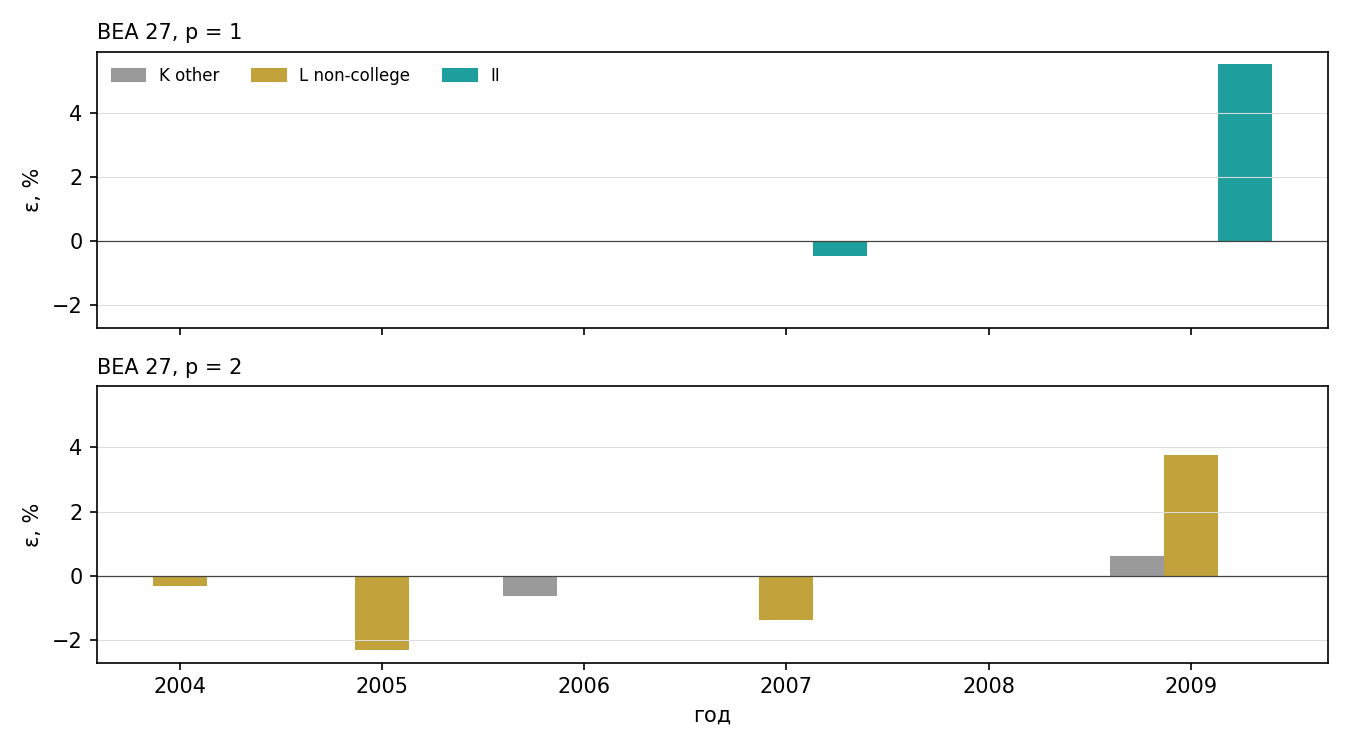
\includegraphics[width=0.9\textwidth]{p1p2_bea27.png}
\caption{BEA 27: относительные сдвиги цен оптимального решения при $p=1$ и $p=2$.}
\label{fig:bea27}
\end{figure}

\begin{figure}[H]
\centering
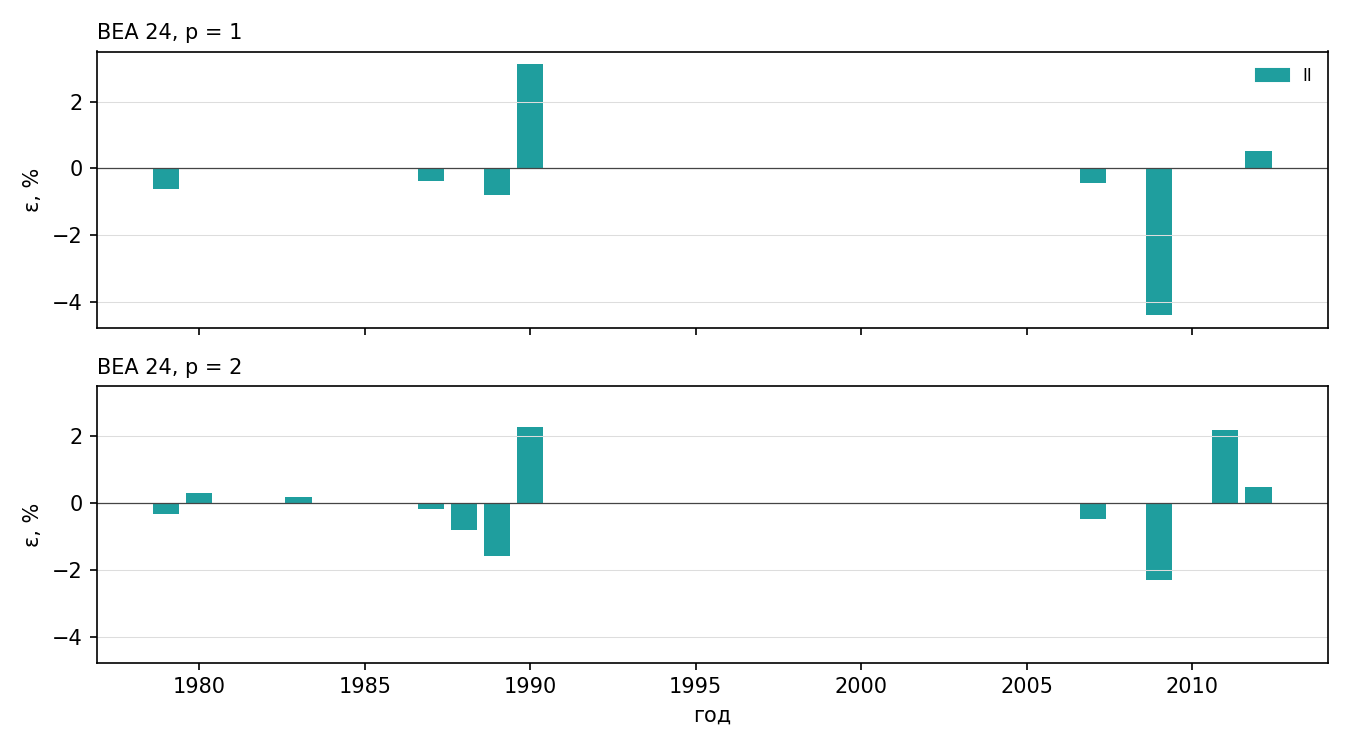
\includegraphics[width=0.9\textwidth]{p1p2_bea24.png}
\caption{BEA 24: относительные сдвиги цен промежуточных товаров при $p=1$ и $p=2$. При $p=2$ каждый разрыв делится между двумя годами.}
\label{fig:bea24}
\end{figure}

\todo{$p=\infty$ на реальных данных; BEA 6 и 31.}

\section{Открытые вопросы}

\begin{enumerate}
    \item Сложность при $d=2$, где оракул полиномиален.
    \item Хватает ли полиномиального числа запросов к оракулу с сертификатами.
\end{enumerate}

\begin{thebibliography}{99}
\bibitem{Cherchye2014} L.~Cherchye, B.~De~Rock, B.~Smeulders, F.~C.~R.~Spieksma. Goodness-of-fit measures for revealed preference tests: complexity results and algorithms. \textit{ACM Trans. Econ. Comput.} 2(1), 2014.
\bibitem{CodatoFischetti2006} G.~Codato, M.~Fischetti. Combinatorial Benders' cuts for mixed-integer linear programming. \textit{Oper. Res.} 54(4):756--766, 2006.
\bibitem{DeanMartin2016} M.~Dean, D.~Martin. Measuring rationality with the minimum cost of revealed preference violations. \textit{Rev. Econ. Stat.} 98(3):524--534, 2016.
\bibitem{DemuynckRehbeck2023} T.~Demuynck, J.~Rehbeck. Computing revealed preference goodness-of-fit measures with integer programming. \textit{Econ. Theory} 76(4):1175--1195, 2023.
\bibitem{FischettiSalvagninZanette2010} M.~Fischetti, D.~Salvagnin, A.~Zanette. A note on the selection of Benders' cuts. \textit{Math. Program.} 124:175--182, 2010.
\bibitem{Tuy2000} H.~Tuy. Monotonic optimization: problems and solution approaches. \textit{SIAM J. Optim.} 11(2):464--494, 2000.
\bibitem{Tuy2005} H.~Tuy. Robust solution of nonconvex global optimization problems. \textit{J. Global Optim.} 32:307--323, 2005.
\bibitem{TuyAlKhayyalThach2005} H.~Tuy, F.~Al-Khayyal, P.~T.~Thach. Monotonic optimization: branch and cut methods. In: \textit{Essays and Surveys in Global Optimization}, Springer, 2005, 39--78.
\bibitem{Varian1985} H.~R.~Varian. Non-parametric analysis of optimizing behavior with measurement error. \textit{J. Econometrics} 30:445--458, 1985.
\end{thebibliography}

\end{document}
